% !Mode:: "TeX:UTF-8"
\chapter{Обзор методов построения тестовых программ - плохое название!}
%Обзорная глава, постановка задачи}

\section{Методы генерации тестовых программ для тестовых шаблонов}

\subsection{Разработка генераторов тестовых программ вручную}

В Институте системного программирования РАН группой под руководством
Александра Камкина разработана технология системного функционального
тестирования микропроцессоров с использованием тестовых
шаблонов~\cite{kamkin, vorobyev}. Построение тестовых шаблонов
осуществляется полуавтоматически на основе тестового покрытия по
модели системы инструкций микропроцессора. Тем самым гарантированно
обеспечивается заданная метрика качества тестирования. Тестовые
шаблоны представляются в виде последовательностей инструкций с
зависимостями между их аргументами (например, <<запись-чтение>>) и
тестовыми ситуациями для инструкций.

Для получения тестовых программ по сгенерированным тестовым шаблонам
следует реализовать на языке Java \emph{конструкторы тестовых
данных}. Под <<тестовыми данными>> понимаются значения регистров,
аргументы инструкций обращения к памяти для инициализации состояния
кэш-памяти и ячеек оперативной памяти, если это требуется. Все
зависимости в тестовом шаблоне обладают направлением,
конструирование аргументов инструкций производится итеративно,
начиная с инструкций, от которых не зависят от еще не обработанные
инструкции. Для выбора независимых значений используется случайная
генерация.

%//плюсы: возможность сгенерировать специальные крайние программы,
%минусы: сложно добиться хорошего покрытия при большом количестве
%зависимостей, потому как для этого надо писать нетривиальные
%конструкторы

\subsection{Комбинаторные методы генерации тестовых программ}

Тестовый шаблон состоит из заданной последовательности инструкций,
аргументами которых являются переменные величины. Кроме того для
каждой переменной величины указывается конечная область значений.
Все значения в области равноправны. Тестовая программа содержит ту
же последовательность инструкций, а для каждого аргумента выбрано
значение из области значений этого аргумента. В комбинаторных
методах инструкции воспринимаются лишь как синтаксические объекты
(термы) -- у них есть лишь имя и аргументы (возможно
типизированные).

Последовательность инструкций может быть задана неявно, но у каждой
инструкции всё же будут переменные величины в качестве аргументов и
для каждой переменной величины задана область значений.
Исследователи из Fujitsu Lab.~\cite{TSE} предлагается описать
последовательность инструкций в виде выражений (Test Specification
Expressions, TSE), а семантику инструкций -- на языке
ISDL~\cite{ISDL}. Отдаленно TSE могут напоминать регулярные
выражения, где бесконечнозначные операции заменены конечными
аналогами. ISDL-описание может включать в том числе и параметры
исполнения инструкции на конвейере, которые могут быть использованы
в TSE. Авторы исследования реализовали специальный генератор,
который строит тестовые программы, удовлетворяющие данному TSE.

Kohno и Matsumoto~\cite{mVpGen} рассматривают задачу верификации
конвейерных микропроцессоров, используя для её решения генерацию
тестовых программ с помощью тестовых шаблонов. Тестовый шаблон явно
содержит последовательность типов инструкций, возможно, с
использованием конструкций итерирования блоков инструкций
(предполагается, что исполнение инструкции на конвейере зависит от
типа инструкции, поэтому, используя обход конечной модели конвейера,
алгоритм генерирует последовательности типов инструкций, т.е.
тестовые шаблоны). Использование разными инструкциями в шаблоне
одной и той же переменной величины должно приводить в тестовой
программе к использованию одного и того же значения для этой
переменной величины. Областями значений являются заданное в
архитектуре множество регистров ($GPR$ -- множество регистров общего
назначения, $CPR$ -- множество регистров сопроцессора). Выбор во
множестве значений осуществляется псевдослучайным образом.

%// плюсы:простота, минусы: низкое покрытие

\subsection{Генерация тестовых программ с использованием методов
решения задачи ATPG}

Задача ATPG (Automatic Test Pattern Generation)~\cite{ATPGbook}
относится к вопросам модульного тестирования микропроцессоров.
Модульное тестирование осуществляется подачей определенных сигналов
(возможно, многотактовых) на входы модуля (схемы) и снятие значения
выходных сигналов (возможно, также многотактовых). Принятие вердикта
осуществляется на основе сравнения ожидаемого выходного сигнала и
снимаемого с данной схемы. Тестовым воздействием является сигнал,
поданный на входные порты схемы. Моделью ошибки является смена
функции некоторых элементов схемы (например, в результате пробоя или
замыкания элемент может сменить функцию, которую он реализует, на
тождественную константу). ATPG -- это задача построения тестовых
воздействий для схем, нацеленных на данную модель ошибки. Аргументы
инструкций являются входными сигналами некоторых модулей
микропроцессора, поэтому решая задачу генерации входных сигналов,
можно решать и задачу генерации тестовых программ.

Эту идею использовали исследователи из Politecnico di
Milano~\cite{toATPG}. Тестовым шаблоном выступает
препроцессированная модель этапа декодирования инструкции. Модель
написана на языке VHDL~\cite{VHDL}. Специальный генератор
подставляет на место кода инструкции заданные значения кодов
операций и передает получившуюся модель стороннему (коммерческому)
ATPG-инструменту. Тот в свою очередь возвращает остальные значения,
которые надо передать в модуль декодирования инструкции, т.е.
значения аргументов инструкции. Метод был применен к тестированию
АЛУ VLIW-микропроцессора.

%//плюсы:позволяет нацеливаться на покрытие по RTL-модели, минусы:
%нужна RTL-модель, небольшая длина тестового шаблона

\subsection{Генерация тестовых программ с использованием методов
разрешения ограничений}

Под \emph{ограничением} будет пониматься предикат, в котором
переменные принимают значения из конечного множества (\emph{домена переменной}). Например, <<$x >
0$>> при $x \in \{0, 10, 100\}$ является ограничением. Задачей разрешения ограничений
(constraint satisfaction problem) является задача поиска значений
для переменных из их доменов, при которых все ограничения
выполнены (предикаты принимают истинное значение)~\cite{CSP}. Для доментов небольшого размера
достаточно перебрать все комбинации значений переменных, пока не
встретится комбинация, на которой выполнены все ограничения. В общем
случае применяются более сложные алгоритмы (зачастую с привлечением
эвристик), сочетающие перебор с возвратом и распространение
ограничений (т.е. автоматический вывод ограничений-следствий по
данной системе ограничений).

Представление в виде CSP~\cite{CSP} удобно для задач,
сформулированных в виде задачи выполнимости некоторого набора
условий. Задача генерации тестовых программ по тестовым шаблонам
тоже может быть сформулирована в таком виде, поскольку есть
связанный набор переменных (инструкций, аргументов инструкций,
элементов состояния микропроцессора), причем связи выражаются в виде
утверждений, зависимостей. Сама идея построения тестовой программы
через формулирование тестового шаблона близка решению задачи с
использованием CSP, поскольку этап построения тестового шаблона
(формализации требований к тестовому воздействию) по сути является
этапом формулирования задачи построения тестового шаблона в виде
утверждений, в виде задачи выполнимости. Остается только перевести
эту формулировку к виду, используемому в инструментах для решения
CSP. Выбор инструментов, методов решения CSP, а также вида самих
ограничений, зависит от того, какие применяются тестовые шаблоны и
как описывается семантика инструкций.

С целью упрощения подготовки нужного представления семантики
микропроцессора китайские исследователи в своем инструменте
\textsc{MAATG}~\cite{MAATG} предложили использовать хорошо известный
язык описания архитектуры EXPRESSION~\cite{EXPRESSION}. Тестовые
шаблоны позволяют явно задавать блоки инструкций, задавать
ограничения на аргументы разных инструкций (одинаковые регистры,
разные регистры, непосредственные значения из некоторого множества
констант), а также указывать события, которые могут произойти при
исполнении инструкции (например, целочисленное переполнение для
инструкции ADD). Специальный генератор строит тестовую программу
итеративно. Сначала он упорядочивает инструкции так, чтобы
переменные для очередной инструкции зависели только от переменных
предыдущих инструкций. Это позволяет разбить задачу генерации
тестовой программы на последовательность более простых задач
генерации одной инструкции. Однако по доступным публикациям
невозможно сделать вывод о том, какие ограничения генерирует MAATG и
тем самым оценить эффективность работы этого инструмента.

Группа американских исследователей, начиная с 1997 года,
разрабатывает инструмент для генерации тестовых программ по тестовым
шаблонам \textsc{RAVEN}~\cite{RAVEN}. Тестовые шаблоны позволяют
задавать свойства последовательности инструкций (заданная
последовательность инструкций, заданная последовательность типов
инструкций, возможно, с указанием вероятности выбора тех или иных
инструкций), зависимости по регистрам. Каждая инструкция может
\emph{изменить контекст}, в том числе и произвести изменение
кэш-памяти. Инструмент не содержит механизма для задания архитектуры
тестируемого микропроцессора пользователем. Вместо этого
подготовлено семейство инструментов для таких архитектур как MIPS,
ARM, POWER. Предполагается, что система инструкций тестируемого
микропроцессора совпадает с системой инструкций одной из этих
архитектур. Инструмент является коммерческим, поэтому в открытых
публикациях практически отсутствует информация о том, каким образом
осуществляется построение тестовых программ. Утверждается, что
используется разрешение ограничений и псевдослучайная генерация.

Еще одно семейство инструментов генерации тестовых программ на
основе тестовых шаблонов было разработано в IBM в течение последних
20 лет. Далее будет дано описание последнего на сегодняшний день
инструмента в этом семействе --
\textsc{Genesys-Pro}~\cite{GenesysPro2004}. Тестовые шаблоны этого
инструмента позволяют описывать как заданные последовательности
инструкций, так и всевозможные их композиции. Разработчиками
предложен несложный императивный язык, позволяющий задать эту
последовательность инструкций.

Для каждой инструкции могут быть указаны ограничения на аргументов
пожелания к значениям аргументов инструкции для улучшения тестового
покрытия (эта информация называется testing
knowledge)~\cite{GenesysTK}. Эти пожелания (по сути особенности
семантики инструкций и тестовые ситуации) предлагается описывать с
использованием ограничений~\cite{GenesysPro2004Innovations}. Можно
задавать ограничения на атрибуты аргументов инструкции (например,
значение одного аргумента больше значения другого) и состояние
микропроцессора (например, на значения в таблицах и буферах). Для
описания механизма трансляции адресов (получения физического адреса
по виртуальному) предлагается использовать подход
DeepTrans~\cite{DeepTrans}. В этом подходе предлагается пользователю
описать структуру строки таблицы, через которую осуществляется
трансляция, правило соответствия адреса строке, некоторые другие
преобразования, а специальный генератор автоматически построит
нужную систему ограничений для использования в \textsc{Genesys-Pro}.

Тестовый шаблон может содержать параметры работы генератора тестовых
программ: вероятности выбора тех или иных значений, параметры
распределения адресов в памяти и другие -- они позволяют управлять
выбором некоторого одного значения из множества допустимых.

Требуется описать структуру системы команд (architecture model),
задать исполнительную семантику команд (по сути симулятор
микропроцессора).

Рассмотрим теперь, как \textsc{Genesys-Pro} генерирует тестовые
программы на основе тестовых шаблонов. Для б\'{о}льшей эффективности
этапы построения последовательности инструкций и выбора аргументов
осуществляются вместе (отдельная инициализация состояния
микропроцессора не проводится). На основе параметров генерации,
текущего состояния модели микропроцессора и построенной тестовой
программы выбирается очередная инструкция (тестовые шаблоны
позволяют описывать сложные потоки управления на инструкциях). Далее
для этой инструкции генерируются аргументы инструкций. Для этого
строится и разрешается система ограничений на основе тестовых
ситуаций (testing knowledge) и текущего модельного состояния
микропроцессора), в результате чего получаются значения аргументов.
Готовая инструкция исполняется на модели микропроцессора
(architecture model, он готовится пользователем) с получением нового
модельного состояния микропроцессора. На этом генерация инструкции
завершается и генерируется следующая инструкция. Ключевым моментом
является эффективность работы решателя ограничений. Для этой цели
разработчики инструмента самостоятельно написали свой решатель
ограничений. Он базируется на хорошо известном семействе алгоритмов
разрешения ограничений MAC (Maintaining Arc-Consistency)~\cite{CSP},
но заточен под ограничения, генерируемые для тестовых
программ~\cite{GenesysSolver}. Написание такого решателя является
довольно нетривиальной задачей и предметом отдельного исследования.
Например, \textsc{Genesys-Pro} позволяет использовать для описания
тестовых ситуаций элементы массивов (Memory, таблицы страниц) с
переменными индексами.

Тем самым ни один из методов генерации тестовых программ,
использующих ограничения, не нацеливается на строго заданную
последовательность инструкций, однако потребности в использовании
тестовых шаблонов с заданной последовательностью инструкций
отмечаются исследователями~\cite{kamkin}.

%//плюсы: масштабируемость, технологичность; минусы: сложность
%внесения нового архитектурного механизма

\subsection{Сравнение методов генерации тестовых программ}

%%%Сравнение проводилось по следующим критериям:
%%%\begin{enumerate}
%%%\item выразительная мощность тестовых шаблонов;
%%%\item допустимые архитектурые механизмы;
%%%\item сложность подготовки исходных данных;
%%%\item переиспользуемость частей генератора тестовых программ;
%%%\item вычислительная эффективность генератора тестовых программ.
%%%\end{enumerate}
%%%
%%%\subsubsection{Выразительная мощность тестовых шаблонов}
%%%\noindent {\small
%%%\begin{tabular}{|l|c|c|c|c|}
%%%\hline &
%%%\begin{tabular}{c}ручная\\генерация\end{tabular} &
%%%\begin{tabular}{c}комбина-\\торные\\методы\end{tabular} &
%%%\begin{tabular}{c}использование\\ATPG\end{tabular} &
%%%\begin{tabular}{c}использование\\CSP\end{tabular} \\
%%%\hline
%%%\begin{tabular}{l}возможность\\задать\\последовательность\\инструкций \end{tabular} &
%%%+ & + & -- & + \\
%%%\hline
%%%\begin{tabular}{l}возможность\\задать\\тестовую\\ситуацию \end{tabular} &
%%%+ & -- & -- & + \\
%%%\hline
%%%\begin{tabular}{l}возможность\\задействовать\\состояние\\микропроцессора \end{tabular} &
%%%+ & -- & + & + \\
%%%\hline
%%%\end{tabular}}
%%%
%%%//нужен комментарий, почему заполнение такое?
%%%
%%%\subsubsection{Допустимые архитектурные механизмы}
%%%\noindent {\small \begin{tabular}{|l|c|c|c|c|} \hline &
%%%\begin{tabular}{c}ручная\\генерация\end{tabular} &
%%%\begin{tabular}{c}комбинаторные\\методы\end{tabular} &
%%%\begin{tabular}{c}использование\\ATPG\end{tabular} &
%%%\begin{tabular}{c}использование\\CSP\end{tabular} \\
%%%\hline
%%%\begin{tabular}{l}поддержка\\регистров\\общего\\назначения \end{tabular} &
%%%+ & + & -- & + \\
%%%\hline
%%%\begin{tabular}{l}поддержка\\кэш-памяти и \\трансляции\\адресов \end{tabular} &
%%%+ & -- & -- & + \\
%%%\hline
%%%\begin{tabular}{l}поддержка\\механизмов\\параллелизма \end{tabular} &
%%%+ & + & -- & + \\
%%%\hline
%%%\end{tabular}}
%%%
%%%//нужен комментарий, почему заполнение такое?
%%%
%%%\subsubsection{Сложность подготовки исходных данных}
%%%\noindent{\small
%%%\begin{tabular}{|l|c|c|c|c|}
%%%\hline &
%%%\begin{tabular}{c}ручная\\генерация\end{tabular} &
%%%\begin{tabular}{c}комбинаторные\\методы\end{tabular} &
%%%\begin{tabular}{c}использо-\\вание\\ATPG\end{tabular} &
%%%\begin{tabular}{c}использование\\CSP\end{tabular} \\
%%%\hline
%%%\begin{tabular}{l}при смене\\тестового\\шаблона \end{tabular} &
%%%сложно & \begin{tabular}{c}сложно\\(нужна\\RTL-модель)\end{tabular} & -- & несложно \\
%%%\hline
%%%\begin{tabular}{l}при смене\\микро-\\процессора \end{tabular} &
%%%\begin{tabular}{c}долго, но\\технологично\end{tabular} &
%%%\begin{tabular}{c}долго\\вплоть до\\невозможности\end{tabular} &
%%%просто & \begin{tabular}{c}небыстро\\(новые\\механизмы)\end{tabular} \\
%%%\hline
%%%\end{tabular}}
%%%
%%%//нужен комментарий, почему заполнение такое?
%%%
%%%\subsubsection{Переиспользуемость частей генератора тестовых
%%%программ} \noindent{\small
%%%\begin{tabular}{|l|c|c|c|c|}
%%%\hline &
%%%\begin{tabular}{c}ручная\\генерация\end{tabular} &
%%%\begin{tabular}{c}комбинаторные\\методы\end{tabular} &
%%%\begin{tabular}{c}использование\\ATPG\end{tabular} &
%%%\begin{tabular}{c}использование\\CSP\end{tabular} \\
%%%\hline
%%%\begin{tabular}{l}при смене\\тестового\\шаблона \end{tabular} &
%%%никакая & полная & полная & полная \\
%%%\hline
%%%\begin{tabular}{l}при смене\\микро-\\процессора \end{tabular} &
%%%никакая & полная &
%%%полная & \begin{tabular}{c}только\\общие\\механизмы\end{tabular} \\
%%%\hline
%%%\end{tabular}}
%%%
%%%//нужен комментарий, почему заполнение такое?
%%%
%%%\subsubsection{Вычислительная эффективность генератора тестовых
%%%программ}
%%%
%%%\noindent {\small
%%%\begin{tabular}{|l|c|c|c|c|}
%%%\hline &
%%%\begin{tabular}{c}ручная\\генерация\end{tabular} &
%%%\begin{tabular}{c}комбина-\\торные\\методы\end{tabular} &
%%%\begin{tabular}{c}использо-\\вание\\ATPG\end{tabular} &
%%%\begin{tabular}{c}использо-\\вание\\CSP\end{tabular} \\
%%%\hline
%%%\begin{tabular}{l}сложность\\достижения\\покрытия \end{tabular} &
%%%\begin{tabular}{c}сложно\\(можно достичь\\крайние случаи)\end{tabular} &
%%%\begin{tabular}{c}сложно\\(не задается\\семантика)\end{tabular} &
%%%\begin{tabular}{c}возможно\\покрытие\\структуры\\RTL-модели\end{tabular} &
%%%несложно \\
%%%\hline
%%%\begin{tabular}{l}среднее время\\генерации\\программ \end{tabular} &
%%%долго & быстро &
%%%\begin{tabular}{c}зависит от\\сложности\\RTL-модели\end{tabular} &
%%%недолго \\
%%%\hline
%%%\begin{tabular}{l}эффективность\\учёта начального\\состояния\\микропроцессора\end{tabular} &
%%%сложно & \begin{tabular}{c}не\\учитывается\end{tabular} &
%%%\begin{tabular}{c}не\\учитывается\end{tabular} &
%%%возможно \\
%%%\hline
%%%\end{tabular}}
%%%
%%%//нужен комментарий, почему заполнение такое?

Сравнение проводилось по следующим критериям:
\begin{enumerate}
\item сложность построения генератора тестовых программ;
\item допустимые архитектурые механизмы;
\item полнота метода.
\end{enumerate}

Из сделанного обзора следует, что возможность генерирования тестовых
программ для тестовых шаблонов, ориентированных на поведение MMU
(тестовые ситуации в кэширующих буферах и таблицах MMU), т.е.
поддержку механизмов кэширования в MMU, есть у следующих методов:
\begin{itemize}
  \item разработка генераторов тестовых программ вручную~\cite{kamkin};
  \item покомандный перебор с возвратом на основе разрешения
  ограничений~\cite{GenesysPro}.
\end{itemize}
Сюда же можно добавить вероятностные алгоритмы генерации тестовых программ (как разновидность
  -- переборные алгоритмы); среди них можно выделить простые
  вероятностные алгоритмы (типа метода
  Монте-Карло~\cite{MonteKarlo}) и более сложные вероятностные
  алгоритмы (например, перебор с обратной связью~\cite{DART}). Хотя в литературе не замечены статьи, где бы этот метод применялся для генерации тестовых программ по тестовым шаблонам, но исключать такие методы тоже нельзя.

Выразительные возможности тестовых шаблонов в остальных методах не позволяют выразить особенности функционирования MMU.

Выделенные методы сравним по критериям сложности построения генераторов и полноты:

\begin{table}[h]\small
\begin{tabular}{|c||c|c|}\hline
 & полный & неполный\\
\hline \hline
простой & & \begin{tabular}{c}переборный алгоритм\\
простой вероятностный \end{tabular} \\
\hline
сложный & \begin{tabular}{c}вручную написанный генератор\\
сложный вероятностный\\покомандный перебор с возвратом
 \end{tabular} & --- \\ \hline
\end{tabular}

\end{table}

Использование простых переборных или вероятностных алгоритмов
генерации тестовых программ позволяют подготовить генератор на
основе очевидных несложных идей, однако они не позволяют добиться
достаточной полноты генерации тестовых программ. Это означает, что
для произвольного тестового шаблона время генерации тестовой
программы может быть очень велико.

Напротив более сложные варианты вероятностных (переборных)
алгоритмов, написанные вручную генераторы или генераторы, основанные
на более регулярных алгоритмах (например, покомандный перебор с
возвратом, реализованный в системе Genesys-Pro~\cite{GenesysPro}),
нацелены на получение высокой полноты. Однако достигается это в
основном за счет разработки и применения уникальных идей, которые
сложно использовать вновь при тестировании другого микропроцессора.
Это усложняет написание таких генераторов и, как результат,
увеличивает время подготовки самого генератора.

В результате экспериментов~\cite{vorobyev} была показана возможность
построения тестовых программ для шаблонов из 2-3 инструкций. Тем не
менее существуют ситуации в работе модулей управления памятью, для
создания которых необходимо больше инструкций (до 8-16). Например,
такие ситуации могут возникать в работе буферов очередей
кэш-промахов~\cite{HennesyPatterson}. Такие буферы применяются для
реализации неблокирующих конвейеров с целью продолжать работу с
кэш-памятью даже при возникновении кэш-промаха (а именно, при
возникновении кэш-промаха необходимо выполнить некоторые действия по
изменению состояния кэш-памяти, которые впрочем затрагивают лишь
ограниченную часть кэш-памяти, а с остальной частью кэш-памяти можно
производить действия параллельно с обработкой кэш-промаха). Для
создания таких ситуаций могут потребоваться тестовые программы,
длина которых сопоставима с длиной буфера очереди кэш-промахов. В
современных микропроцессорах встречаются буферы очереди
кэш-промахов, длины которых равны 8~\cite{Alpha21264} или
16~\cite{Alpha21364, Cell}. Тем самым для тестирования модулей
управления памяти недостаточно представленных доступных методов,
поскольку они не дают возможности построить тестовые программы для
нужных тестовых шаблонов большей длины.

Тем самым представляется перспективным исследование и разработка
регулярных легко переиспользуемых методов построения генераторов
тестовых программ по тестовым шаблонам, применимых для тестирования
механизмов кэширования, не уступающих в полноте существующим
методам.

%\section{Генераторы тестовых данных для абстрактных тестовых
%воздействий}
%
%Рассмотрим работы по генерации тестовых данных для тестовых
%воздействий, которые задаются \emph{в абстрактном виде}. А именно, в
%виде требований на аргументы вызываемых в тестовом воздействии
%функций системы. Одним из примеров таких абстрактных тестовых
%воздействий являются тестовые шаблоны, поскольку они задают
%требования на аргументы инструкций, входящих в тестовую программу.
%Другим примером абстрактных тестовых воздействий являются
%\emph{параметрические тесты}~\cite{Pex} для программных систем. Они
%напоминают модульные тесты (unit-тесты), в которых аргументы
%вызываемых методов могут быть переменными величинами.
%
%\subsection{Симуляционные методы}
%Идея симуляционных методов (simulation-based) состоит в чередовании
%этапов разрешения ограничений и исполнения кода (<<симуляции>>).
%Рассмотрим абстрактное тестовое воздействие в виде
%последовательности чередующихся инструкций $i_1, i_2, \dots, i_N$ и
%условий пути $P_1, P_2, \dots, P_N$:
%$$
%\begin{array}{l}
%\mbox{condition: } P_1(x_1, x_2, \dots, x_{n_1})\\
%\mbox{instruction: }i_1 (x_1, x_2, \dots, x_{n_1})\\
%\mbox{condition: } P_2 (x_1, x_2, \dots, x_{n_1}, x_{n_1+1}, \dots, x_{n_2})\\
%\mbox{instruction: }i_2 (x_1, x_2, \dots, x_{n_2})\\
%\mbox{condition: } P_3(x_1, x_2, \dots, x_{n_2}, x_{n_2+1}, \dots, x_{n_3})\\
%\mbox{instruction: }i_3 (x_1, x_2, \dots, x_{n_3})\\
%\dots\\
%\mbox{instruction: }i_N (x_1, x_2, \dots, x_n)\\
%\end{array}
%$$
%
%Для каждой инструкции определен \emph{симулятор}, т.е. процедура,
%которая позволяет исполнить инструкцию с некоторыми значениями
%аргументов. Каждое условие пути задано формулой в некотором языке.
%Ключевым моментом является отсутствие трактовки инструкции как
%отношения на параметрах-результатах и параметрах-значениях.
%
%Тестовыми данными являются значения $x_1, x_2, \dots, x_n$. Их поиск
%осуществляется с помощью следующего перебора с
%возвратом~\cite{GenesysPro}: для $i$'й инструкции составляются и
%разрешаются ограничения из условия пути перед этой инструкцией с
%учетом уже известных значений тестовых данных и текущего модельного
%состояния системы; если составленная система ограничений совместна,
%то входящие в нее тестовые данные получают значение; если
%составленная система ограчения несовместна, происходит возврат на
%предыдущий шаг для выбора других значений тестовых данных. Как
%только для инструкции получены значения аргументов, запускается
%симулятор этой инструкции для получения нового модельного состояния
%системы. На этом принципе основаны инструменты семейства
%Genesys-Pro~\cite{GenesysPro}.
%
%Этот метод обладает хорошей масштабируемостью, поскольку в нем
%разделяется задача поиска значений $x_1, x_2, \dots, x_n$ на поиск
%значений меньшего числа переменных. Этот метод подходит для сложных
%систем, поскольку не возникает необходимости в составлении и
%разрешении ограничений для всего тестового воздействия.
%
%Однако разработчики Genesys-Pro столкнулись с тем, что даже такое
%упрощение ограничений не позволяет использовать для разрешения
%ограничений обычные используемые решатели широкого
%назначения~\cite{CLPusingECLiPSe}. Им пришлось разрабатывать
%специальные алгоритмы и эвристики для подготовки решателя,
%способного решать ограничения того вида, которые генерирует
%Genesys-Pro~\cite{GenesysSolver}. Побочным эффектом этого стал
%низкий процент переиспользования кода при построении решателя
%ограничений для новой архитектуры микропроцессоров.
%
%\subsection{Генерация с использованием символьного исполнения}
%Идеей методов, использующих символьное исполнение (symbolic
%execution), является составление единой системы ограничений для
%всего тестового воздействия. Благодаря появлению в последние годы
%общедоступных решателей ограничений~\cite{Z3, Yices}, появляются и
%инструменты генерации тестовых воздействий, среди которых можно
%выделить Pex~\cite{Pex}. Например, для того же абстрактного
%тестового воздействия
%$$
%\begin{array}{l}
%\mbox{condition: } P_1(x_1, x_2, \dots, x_{n_1})\\
%\mbox{instruction: }i_1 (x_1, x_2, \dots, x_{n_1})\\
%\mbox{condition: } P_2 (x_1, x_2, \dots, x_{n_1}, x_{n_1+1}, \dots, x_{n_2})\\
%\mbox{instruction: }i_2 (x_1, x_2, \dots, x_{n_2})\\
%\mbox{condition: } P_3(x_1, x_2, \dots, x_{n_2}, x_{n_2+1}, \dots, x_{n_3})\\
%\mbox{instruction: }i_3 (x_1, x_2, \dots, x_{n_3})\\
%\dots\\
%\mbox{instruction: }i_N (x_1, x_2, \dots, x_n)\\
%\end{array}
%$$
%для получения значений переменных $x_1, x_2, \dots, x_n$ будет
%построена следующая система ограничений:
%$$
%\left\{\begin{array}{l}
%P_1(x_1, x_2, \dots, x_{n_1})\\
%I_1 (x_1, x_2, \dots, x_{n_1})\\
%P_2 (x_1, x_2, \dots, x_{n_1}, x_{n_1+1}, \dots, x_{n_2})\\
%I_2 (x_1, x_2, \dots, x_{n_2})\\
%P_3(x_1, x_2, \dots, x_{n_2}, x_{n_2+1}, \dots, x_{n_3})\\
%I_3 (x_1, x_2, \dots, x_{n_3})\\
%\dots\\
%I_N (x_1, x_2, \dots, x_n)\\
%\end{array}\right.
%$$
%в которой отношение $I_k(x_1, x_2, \dots, x_{n_k})$ описывает
%отношение параметров-результатов и параметров-значений среди
%аргументов инструкции $i_k$ и получено путем символьного исполнения
%инструкции $i_k$~\cite{symbolic_execution}.
%
%Из-за своей природы масштабируемость этих методов зависит от
%эффективности работы решателя ограничений. Сложности возникают и при
%генерации тестовых данных <<сложной природы>>: деревья, графы,
%особые списки.
%
%Тем не менее пока не было показана возможность и сущность применения
%символьного исполнения для построения тестовых программ по тестовым
%шаблонам, что представляется перспективным.

\section{Постановка задачи}

В диссертации решается задача построения тестовых программ по
тестовым шаблонам, обладающим следующими свойствами.

\emph{Тестовым шаблоном} называется последовательностью троек $(I_i,
A_i, S_i)$, где:
\begin{itemize}
  \item $I_i \in \mathcal{I}$ -- инструкция из множества инструкций
микропроцессора $\mathcal{I}$;
  \item $A_i \in (\mathcal{R} \cup \mathcal{C})^*$ -- список аргументов
  инструкции: аргументом может быть регистр из множества регистров
  микропроцессора $\mathcal{R}$ (явно задано имя регистра) или
  переменная с константным значением ($\mathcal{C}$ -- множество
  переменных); количество аргументов инструкции соответствует
  требуемому в архитектуре микропроцессора;
  \item $S_i \subseteq \mathcal{M}(I_i)$ -- \emph{тестовая ситуация} инструкции -- набор идентификаторов (по сути веьвей функциональности, определяющих происходящие при исполнении инструкции события).
\end{itemize}

$(\mathcal{I},~\mathcal{R},~\mathcal{M})$ составляют \emph{модель микропроцессора}.

Пример тестового шаблона:
\begin{verbatim}
ADD r1, r2, r3 @ overflow
LW r4, r1, c @ l1Miss, l2Hit
\end{verbatim}
Множество инструкций включает в себя \texttt{ADD} и \texttt{LW}.
Аргументами первой инструкции является список (\texttt{r1, r2, r3}),
второй -- список (\texttt{r4, r1, c}). Тестовой ситуацией первой
инструкции является метка <<overflow>>. Тестовый шаблон не определяет смысл метки, для тестового шаблона важно лишь то, что <<overflow>> имеет отношение к инструкции \texttt{ADD}. Семантика этой инструкции описана в документации по микропроцессору, там же может быть описан и смысл <<overflow>> (например, это может быть возникновение переполнения).
Тестовой ситуацией второй инструкции является <<l1Miss, l2Hit>>. Опять же для тестового шаблона это просто два идентификатора (например, они могут означать, что при исполнении инструкции может произойти кэш-промах в кэш-памяти первого уровня и кэш-попадание в кэш-памяти второго уровня).

\emph{Тестовая программа} -- это последовательность двоек $(I_i,~A'_i)$, где
\begin{itemize}
  \item $I_i \in \mathcal{I}$ -- инструкция из множества инструкций
микропроцессора $\mathcal{I}$;
  \item $A'_i \in (\mathcal{R} \cup \mathds{N})^*$ -- список
  аргументов инструкции: аргументом может быть регистр из множества
  регистров микропроцессора $\mathcal{R}$ (явно задано имя регистра)
  или константа (непосредственное значение); количество аргументов
  инструкции соответствует требуемому в архитектуре микропроцессора.
\end{itemize}

Для определения отношения соответствия тестовых программ тестовым шаблонам опишем \emph{семантику инструкций} как отношение на множестве $(\mathcal{I} \times (\mathcal{R} \cup \mathds{N})^* \times (N(\mathcal{R}) \times \mathcal{S}) \times (N(\mathcal{R}) \times \mathcal{S}) \times \mathcal{M}(\mathcal{I}) \times \mathcal{E})$, где:
\begin{itemize}
  \item $\mathcal{I}$ -- инструкция, для которой определяется семантика;
  \item $(\mathcal{R} \cup \mathds{N})^*$ -- имена аргументов-регистров и значения аргументов-констант инструкции;
  \item $N(\mathcal{R}) \times \mathcal{S}$ -- входные или выходные (встречаются в отношении дважды) значения регистров и состояние внутренних компонент;
  \item $\mathcal{M}(\mathcal{I})$ -- метки инструкции, активировавшиеся при исполнении данной инструкции с данными аргументами в данном состоянии;
  \item $\mathcal{E}$ -- исключение, произошедшее при исполнении инструкции.
\end{itemize}

В результате исполнения тестовой программы получается \emph{трасса исполнения}. Она определяется с использованием семантики инструкций. Под трассой исполнения будем понимать последовательность векторов $(I_i, S'_i)$, где
\begin{itemize}
  \item $I_i$ -- инструкция;
  \item $S'_i$ -- метки инструкции $I_i$, активировавшиеся при ее исполнении.
\end{itemize}

Трасса $R = (I_i, M'_i)^*$ (ее длину обозначим $r$) \emph{соответствует} тестовой программе $P = (I'_j, A'_j)^*$ (ее длину обозначим $p$)  для микропроцессора с системой инструкций, семантика которых задается как отношение $\mathcal{U} \subseteq (\mathcal{I} \times (\mathcal{R} \cup \mathds{N})^* \times (N(\mathcal{R}) \times \mathcal{S}) \times (N(\mathcal{R}) \times \mathcal{S}) \times \mathcal{M}(\mathcal{I}) \times \mathcal{E})$, если одновременно выполнены следующие условия:
\begin{enumerate}
  \item $r = p$;
  \item для всех $i \in \{1, 2, ..., r\}$ $I_i = I'_i$;
  \item для всех $i \in \{1, 2, ..., r\}$ $M'_i \subseteq \mathcal{M}(I_i)$;
  \item для всех $i \in \{1, 2, ..., r\}$ существуют $S''_0, S''_1, E''$ такие, что \\$(I_i, A'_i, S''_0, S''_1, M'_i, E'') \in \mathcal{U}$ (каждый элемент трассы и программы соответствует семантике инструкции).
\end{enumerate}

Тестовая программа $P = (I_i, A'_i)^*$ (ее длину обозначим $p$) с соответствующей ей трассой исполнения $R = (I_i, S'_i)^*$ \emph{соответствует} тестовому шаблону $T = (II_i, AA_i, SS_i)^*$ (его длину обозначим $t$) , если одновременно выполнены следующие условия:
\begin{enumerate}
  \item $p \geqslant t$;
  \item для всех $i \in \{p{-}t{+}1, p{-}t{+}2, ..., p\}$ $I_{i-p+t} = II_i$;
  \item для всех $i \in \{p{-}t{+}1, p{-}t{+}2, ..., p\}$ $A'_{i-p+t}$ соответствует $AA_i$: длины этих последовательностей совпадают и совпадают имена аргументов, т.е. обозначив $\alpha = A'_{i-p+t}$ и $\beta = AA_i$, получим, что для всех допустимых индексов этих последовательностей $k$, если $\beta_k \in \mathcal{R}$, то $\alpha_i = \beta_i$ (имена аргументов-регистров совпадают), в противном случае непосредственное значение $\alpha_i$ имеет одно и то же значение во всех инструкциях, где используется тот же $\beta_i$ (одному аргументу-константе в тестовом шаблоне соответствует одно и то же значение на протяжении всего теста);
  \item для всех $i \in \{p{-}t{+}1, p{-}t{+}2, ..., p\}$ $S'_i \supseteq SS_i$.
\end{enumerate}

Грубо говоря, тестовую программу можно разделить на две составляющие: преамбулу, \emph{инициализирующую программу} (она состоит из \emph{инициализирующих инструкций}), и следующую за ней часть программы (она состоит из \emph{инструкций тестового воздействия}), напрямую соответствующую тестовому шаблону (см.рис.~\ref{problem}). Инициализирующая
программа переводят микропроцессор в некоторое состояние, необходимое для заданного исполнения инструкций тестового шаблона. Эти инструкции в точности повторяют последовательность инструкций тестового шаблона с заменой аргументов-констант на непосредственные значения. На рисунке~\ref{test_template_exmp}
приведен пример тестового шаблона и возможных инструкций тестового
воздействия, построенных по этому шаблону.

\begin{figure}[h] \center
  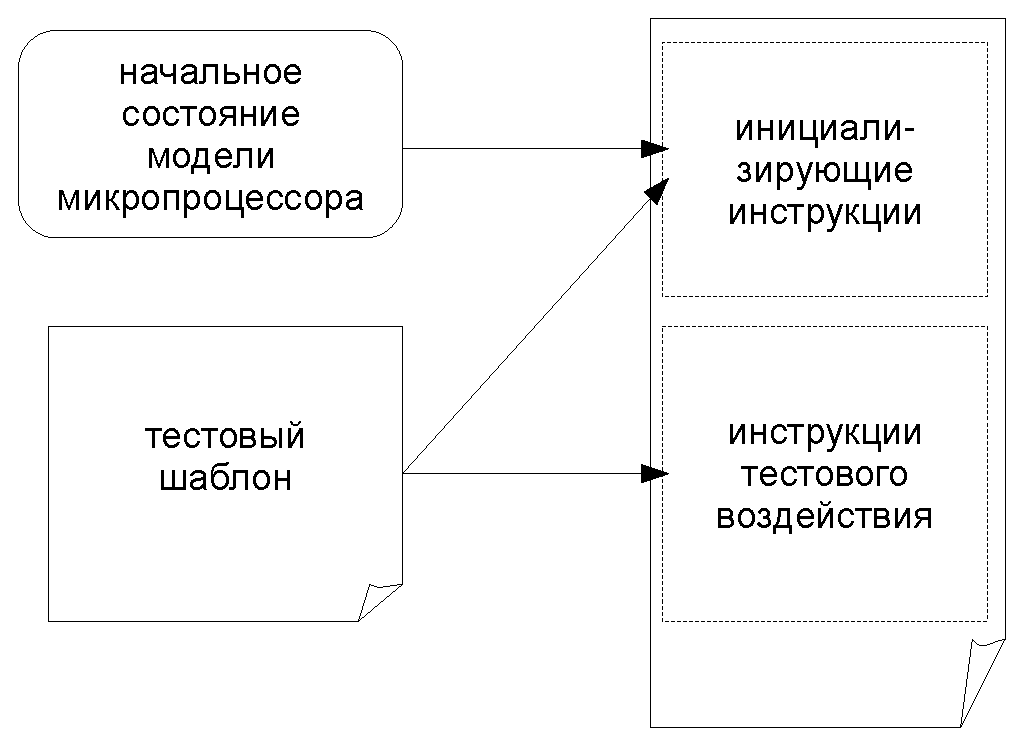
\includegraphics[width=0.5\textwidth]{1.review/problem}\\
  \caption{Составление тестовой программы}\label{problem}
\end{figure}

\begin{figure}[h]
\quad\parbox{0.5\textwidth}{\small \tt
AND r1, r2, r3 @ normal\\
LD r4, r2, c1 @ l1Hit\\
SUB r3, r1, r5 @ overflow } \parbox{0.3\textwidth}{\small \tt
AND r1, r2, r3\\
LD r4, r2, 0x0FA2\\
SUB r3, r1, r5
}
\caption{Тестовый шаблон и возможные соответствующие ему инструкции
тестового воздействия}\label{test_template_exmp}
\end{figure}

Сгенерированная тестовая программа может быть дополнена
инструкциями проверки состояния микропроцессора после исполнения
инструкций тестового воздействия (например, такая программа может сообщать тем или иным способом о несоответствии значения, хранящегося в некотором регистре после исполнения инструкций тестового воздействия).

Рассматриваются следующие варианты постановки задачи:
\begin{itemize}
  \item \emph{по начальному состоянию модели микропроцессора}: оно может быть задано, и в этом случае тест (инициализирующие инструкции) начинает исполняться из этого состояния, или начальное состояние может быть не задано, в этом случае тест должен быть построен так, чтобы он работал из любого начального состояния;
  \item \emph{по форме результата}:  .................
\end{itemize}
заданное/незаданное начальное состояние ;
форма результата - инструкции против дампа памяти ;
представление семантики инструкции - constraint-net ;

\cite{my_isp_2009, my_programmirovanie_2009} куда вставить-то ??


В работе рассматривается модель
микропроцессора, включающая в себя регистры общего назначения,
кэш-память (возможно многоуровневую), различные подсистемы для выполнения
трансляции адресов (TLB)~\cite{HennesyPatterson}.

Решение поставленной задачи для тестовых шаблонов, в которых
$\mathcal{S} = \varnothing$, хорошо известно~\cite{my_syrcose_2008,
my_isp_2008} (тестовые ситуации в таких тестовых шаблонах
формулируются лишь на значения регистров и констант-аргументов
инструкций). Для этого тестовые ситуации транслируются в ограничения
(constraints), а искомые начальные значения регистров и значения
констант получаются в результате разрешения этих
ограничений~\cite{CSP}. Для того, чтобы в тестовых шаблонах
использовать инструкции, аргументы которых связаны (например, должны
быть равны или неравны), кроме ограничения на значения аргументов и
состояние микропроцессора, надо дать определение
аргумента-результата инструкции (задействовать семантику
инструкции). Предметом исследования являются способ построения
ограничений в случае $\mathcal{S} \neq \varnothing$ при разных
способах задания семантики инструкций.

%В данной работе среди методов генерации тестовых программ выбран
%метод, использующий разрешение ограничений~\cite{CSP}. Однако по
%сравнению с существующими аналогами в данной работе поставлена
%задача исследовать возможности снижения сложности подготовки
%генератора тестовых программ (по сравнению, например, с мощным
%Genesys-Pro), не проиграв сильно в масштабируемости генератора. При
%этом, возможно, придется выделить среди всевозможных архитектурных
%механизмов наиболее часто использующиеся и требующие тестирование в
%современных микропроцессорах.


\section{Предварительные сведения и термины}

%Дополнительные сведения, необходимые для дальнейшего прочтения.

\subsection{Типы кэш-памяти}

По организации кэш-память делят на \emph{полностью ассоциативную},
\emph{прямого доступа} и \emph{наборно-ассоциативную}. Различие
производится на основе двух параметров: количества секций $W$ и
количества наборов $R$. Кэш-память хранит некоторый набор данных.
Каждому блоку данных соответствует некоторый адрес (физический или
виртуальный). Блоки с адресами организованы в \emph{секции} и
\emph{наборы} (см.рис.~\ref{cache_model}).

\begin{figure}[h] \center
  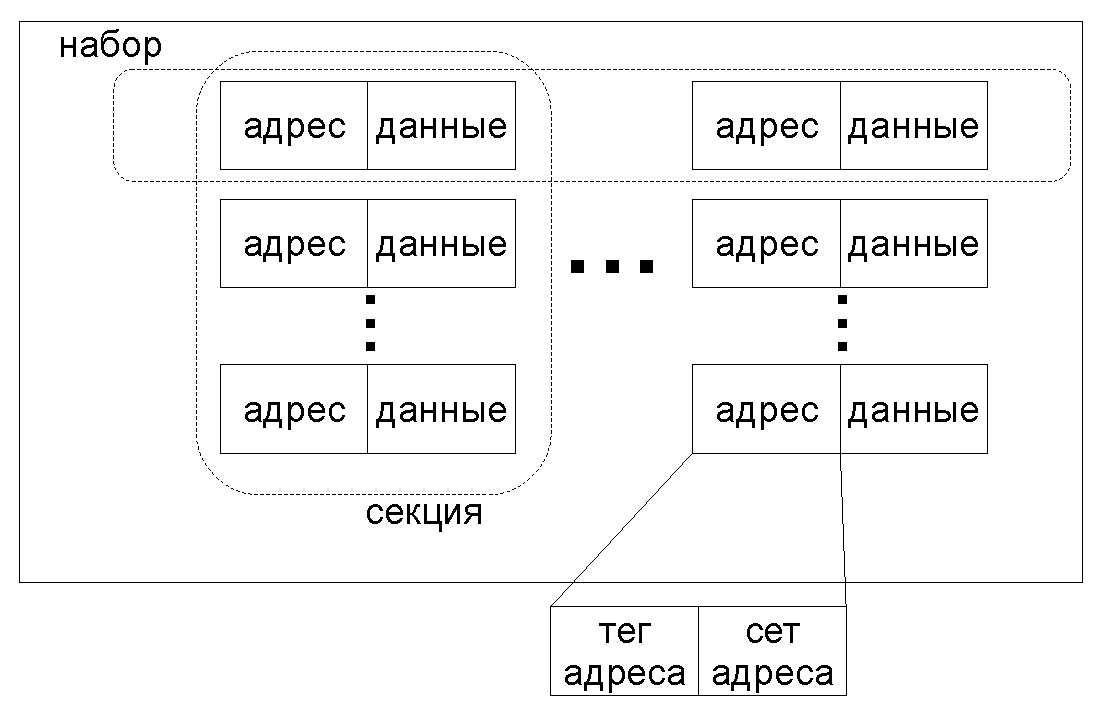
\includegraphics[width=0.7\textwidth]{1.review/cache}\\
  \caption{Модель кэш-памяти и адреса данных}\label{cache_model}
\end{figure}

Каждый адрес может быть разделен на два битовых поля: поле
\emph{тега адреса} и поле \emph{сет адреса}. Один набор составляют
адреса с одинаковым сетом. Кэш-память организована таким образом,
что для каждого сета хранится всегда одно и то же количество адресов
(равное количеству секций $W$). Адреса всех данных в кэш-памяти
различные. Отсюда следует, что теги адресов одного набора разные. В
кэш-памяти представлены все наборы, возможные в рамках битового поля
сета адреса.

Кэш-память является полностью ассоциативной, если $R = 1$.
Кэш-память является кэш-памятью прямого доступа, если $W = 1$. И
кэш-память является наборно-ассоциативной, если $R > 1$ и $W > 1$.

Инструкции обращения в память бывают двух видов: инструкции загрузки
данных из памяти по данному адресу и инструкции сохранения данных в
памяти по данному адресу. При выполнении этих инструкций может быть
задействована кэш-память. Если данные по требуемому адресу
присутствуют в кэш-памяти, операция проводится с нею. Такая ситуация
называется \emph{кэш-попаданием}. Если данные по требуемому адресу
не присутствуют в кэш-памяти, осуществляется подгрузка данных в
кэш-память и совершение операции. Такая ситуация называется
\emph{кэш-промахом}. В этом случае если кэш-память полностью
заполнена, некоторые данные должны быть \emph{вытеснены} из
кэш-памяти и на их место будут загружены данные по требуемому
адресу. \emph{Стратегия вытеснения} (или \emph{политика замещения})
-- это правило, по которому определяются вытесняемые данные.
Например, могут быть вытеснены данные, которые дольше всего не были
нужны (такая стратегия называется \LRU), или данные, которые были
внесены в кэш-память раньше остальных (такая стратегия называется
\FIFO).

\subsection{Таблицы вытеснения}

Для возможности формальных рассуждений о стратегиях вытеснения
потребуется более явное определение стратегии вытеснения нежели
просто <<правило определения вытесняемого тега>>. Для этого
воспользуемся \emph{таблицами вытеснения} (\emph{policy table}). Они
были предложены в 2008 году исследователями из немецкого
университета Саарланда~\cite{policy_tables}. Таблица вытеснения
однозначно описывает изменение порядка и вытеснение тегов в наборе.
Таблица представляет собой матрицу $(w{+}1) \times (w{+}1)$, где $w$
--- ассоциативность кэширующего буфера. Первый столбец ---
специальный, он содержит указание позиций от 0 до $w{-}1$ и
специальную <<псевдопозицию>> для промаха. Остальными элементами
матрицы являются числа от 0 до $w{-}1$ и специальный символ $m$ для
вытесняющего тега. Пример таблицы вытеснения (для стратегии
вытеснения \LRU) смотрите на рисунке~\ref{PolicyTableLRU8}.

\begin{figure}[h]
$$ \left[
     \begin{array}{c|cccccccc}
       \pi_0 & 0 & 1 & 2 & 3 & 4 & 5 & 6 & 7 \\
       \pi_1 & 1 & 0 & 2 & 3 & 4 & 5 & 6 & 7 \\
       \pi_2 & 2 & 0 & 1 & 3 & 4 & 5 & 6 & 7 \\
       \pi_3 & 3 & 0 & 1 & 2 & 4 & 5 & 6 & 7 \\
       \pi_4 & 4 & 0 & 1 & 2 & 3 & 5 & 6 & 7 \\
       \pi_5 & 5 & 0 & 1 & 2 & 3 & 4 & 6 & 7 \\
       \pi_6 & 6 & 0 & 1 & 2 & 3 & 4 & 5 & 7 \\
       \pi_7 & 7 & 0 & 1 & 2 & 3 & 4 & 5 & 6 \\
       \pi_m & m & 0 & 1 & 2 & 3 & 4 & 5 & 6 \\
     \end{array}
   \right]
$$
\caption{Таблица вытеснения для стратегии вытеснения \LRU,
8-ассоциативный кэширующий буфер}\label{PolicyTableLRU8}
\end{figure}

Первые строки таблицы вытеснения описывают изменение порядка
элементов набора при кэш-попаданиях. Каждой такой строке
соответствует свой случай кэш-попадания, при этом первый столбец
показывает, тег с какой позицией дает кэш-попадание, а части строк,
не включающие первый столбец, показывают, каким образом
осуществляется перестановка тегов набор из последовательности
индексов (0 1 ... $w{-}1$). Например, для стратегии вытеснения \LRU,
представленной на рисунке~\ref{PolicyTableLRU8}, при кэш-попадании
тега 5 к набору (4 6 5 7 1 0 2 3) будет применена перестановка
(смотрим строку с $\pi_2$, потому что тег 5 находится на втором
месте) (2 0 1 3 4 5 6 7), что даст следующий порядок элементов
набора: (5 4 6 7 1 0 2 3).

Последняя строка таблицы вытеснения соответствует ситуации
кэш-промаха. Вытесняющий элемент набора помечается буквой $m$.
Вытесняемый элемент -- элемент набора (0 1 ... $w{-}1$), который
отсутствует в последней строке таблицы вытеснения (в примере -- это
7, т.е. вытесняется последний элемент, а вытесняющий помещается на
нулевое место).

В качестве примера приведем таблицы вытеснений для других двух
стратегий вытеснения -- \FIFO и \MRU (см.
рис.~\ref{fig:fifo_mru_tables}).

\begin{figure}[h] \centering
\parbox{0.4\textwidth}{
$$ \left[
     \begin{array}{c|cccccccc}
       \pi_0 & 0 & 1 & 2 & 3 & 4 & 5 & 6 & 7 \\
       \pi_1 & 0 & 1 & 2 & 3 & 4 & 5 & 6 & 7 \\
       \pi_2 & 0 & 1 & 2 & 3 & 4 & 5 & 6 & 7 \\
       \pi_3 & 0 & 1 & 2 & 3 & 4 & 5 & 6 & 7 \\
       \pi_4 & 0 & 1 & 2 & 3 & 4 & 5 & 6 & 7 \\
       \pi_5 & 0 & 1 & 2 & 3 & 4 & 5 & 6 & 7 \\
       \pi_6 & 0 & 1 & 2 & 3 & 4 & 5 & 6 & 7 \\
       \pi_7 & 0 & 1 & 2 & 3 & 4 & 5 & 6 & 7 \\
       \pi_m & m & 0 & 1 & 2 & 3 & 4 & 5 & 6 \\
     \end{array}
   \right]$$
\center \FIFO} \qquad
\parbox{0.4\textwidth}{
$$ \left[
     \begin{array}{c|cccccccc}
       \pi_0 & 1 & 2 & 3 & 4 & 5 & 6 & 7 & 0 \\
       \pi_1 & 0 & 2 & 3 & 4 & 5 & 6 & 7 & 1 \\
       \pi_2 & 0 & 1 & 3 & 4 & 5 & 6 & 7 & 2 \\
       \pi_3 & 0 & 1 & 2 & 4 & 5 & 6 & 7 & 3 \\
       \pi_4 & 0 & 1 & 2 & 3 & 5 & 6 & 7 & 4 \\
       \pi_5 & 0 & 1 & 2 & 3 & 4 & 6 & 7 & 5 \\
       \pi_6 & 0 & 1 & 2 & 3 & 4 & 5 & 7 & 6 \\
       \pi_7 & 0 & 1 & 2 & 3 & 4 & 5 & 6 & 7 \\
       \pi_m & 0 & 1 & 2 & 3 & 4 & 5 & 6 & m \\
     \end{array}
   \right]$$
\center \MRU } \caption{Таблицы вытеснения для 8-ассоциативного
кэширующего буфера}\label{fig:fifo_mru_tables}
\end{figure}

В отличие от определений, в которых теги получали свои позиции и не
меняли их, а критерий вытеснения определялся на основе
дополнительных структур данных, определение с помощью таблицы
вытеснения описывает перестановку тегов в наборе без дополнительных
структур данных.

\subsection{Методы разрешения ограничений}

Задача разрешения ограничений (CSP, Constraint Satisfaction
Problem)~\cite{CSP} определяется с использованием множества
переменных $x_1,~x_2,~\dots,~x_n$, для каждой переменной указана
конечная область значений $D_1,~D_2,~\dots,~D_n$, и отношений на
этих переменных (\emph{ограничений}). Задача состоит в отыскании
значений переменных из своих областей значений, которые
удовлетворяют отношениям на них (см. рис.~\ref{csp}).

\begin{figure}[h] \center
  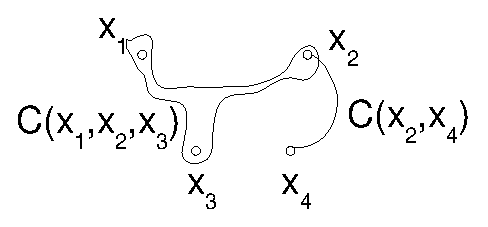
\includegraphics[width=0.5\textwidth]{2.theor/csp}\\
  \caption{Constraint Satisfaction Problem}\label{csp}
\end{figure}

Впервые задача разрешения ограничений в данной формулировке была
предложена Уго Монтанари в 1974 году~\cite{montanari} при решении
задачи машинного зрения. Монтанари ввел понятие сети ограничений
(constraint net) и на основе этой сети предложил метод разрешения
ограничений.

Основной методикой решения CSP является распространение ограничений
(constraint propagation), а именно итеративное построение новых
ограничений на основе данного в задаче множества ограничений
(логических следствий). Если в процессе распространения ограничений
будет построено тождественно ложное ограничение, то CSP является
\emph{несовместной}, для нее не существует решений. Особо обращается
внимание на одноместные ограничения, поскольку с помощью них
уменьшается область значений переменной. Если распространение
ограничений не привело к тождественно ложному ограничению, то в
случае уменьшения области значений некоторой переменной до
единственного значения это значение и будет ответом для данной
переменной. Если же в области определения всё ещё много значений, то
для выбора из области значений используются различные техники
перебора (последовательный перебор, перебор в случайном порядке,
метод ветвей и границ). Эвристические алгоритмы решения CSP обычно
чередуют этапы перебора значений и распространения ограничений.
Одними из таких алгоритмов являются алгоритмы семейства MAC
(Maintaining Arc Consistency)~\cite{CSP}. Другие алгоритмы
перечислены в~\cite{CSPS1},~\cite{CSPS2},~\cite{CSPS3}.

Одним из важных направлений развития CSP стала интеграция с
парадигмой логического программирования. Она позволила динамически
менять множество отношений~\cite{CLPusingECLiPSe}. Примеры систем
CLP (Constraint Logic Programming) -- SICStus Prolog~\cite{SICStus},
ILOG~\cite{ILOG}, ECLiPSe~\cite{CLPusingECLiPSe}. В этих системах
используются стандартные алгоритмы разрешения ограничений для
некоторых типов переменных (а именно, целые числа, вещественные
числа, строки и т.п.).

Задолго до работы Уго Монтанари в 1959 году Мартин Дэвис и Хилари
Путнэм работали в Национальном Агентстве Безопасности над системой
построения доказательств в логике первого порядка~\cite{DPLL}. Через
год появилась публикация алгоритма (\emph{алгоритм
Дэвиса-Патнэм})~\cite{DPLL60}. Он предполагал перебор с возвратом
всех значений переменных, входящих в исследуемую формулу, с
использованием эвристик, сокращающих формулу. Георг Логеманн и
Дональд Ловеланд усовершенствовали этот алгоритм~\cite{DPLL62}.
Результат этого известен как DPLL-алгоритм. Он стал основой для
инструментов разрешения ограничений над пропозициональными
переменными (их области значений состоят лишь из двух значений:
истины и лжи). Такие инструменты известны как
\emph{SAT-инструменты}, например, Chaff~\cite{Chaff} или
WalkSAT~\cite{WalkSAT}.

Вместо поиска единственной разрешающей процедуры для любой формулы
были найдены эффективные разрешающие процедуры для формул для
специальных языках (<<теориях>>). \emph{SMT (Satisfiability Modulo
Theory)} --- задача построения разрешающих процедур для формул
логики первого порядка в некоторой теории. Такие разрешающие
процедуры были найдены для теорий неинтерпретируемых функций с
равенством~\cite{Tveretina}, битовых
строк~\cite{DecisionProcedures}, линейной арифметики (арифметики
Пресбургера)~\cite{OppenNelsonPresburger}, многочленов над
вещественными числами~\cite{DecisionRealPolynomials}, векторов и
многие другие теории. Кроме того было построено несколько методов
построения разрешающих процедур для объединения
теорий~\cite{NelsonOppenProcedure, Shostak, DTC}. Всё это сделало
возможным построение SMT-инструментов~\cite{Z3, Yices} на практике.
В частности были верифицированы некоторые конвейеры и RTL-модели
микропроцессоров~\cite{Bryant, SMT_Circuets, SMT_Pipeline,
MathSAT_RTL}.
